\documentclass[a4paper, 12pt, finnish]{report} %dokumenttiluokka ja sille muutamia määrityksiä
\usepackage[utf8]{inputenc}
\usepackage{mathtools}
\usepackage{amsfonts}
\usepackage{eurosym}
%%\usepackage[toc,page]{appendix}
\usepackage{amsmath} %matematiikka kirjasto
\usepackage{graphicx} %kuvien liittämiseen kuten etusivun Aalto-logo
%\usepackage{pgfplots} %kuvaajien piirtämiseen, ota kommentointi pois mikäli haluat käyttää
\usepackage[finnish]{babel} %suomenkieli
\addto{\captionsfinnish}{\renewcommand{\bibname}{Lähteet}}
\usepackage{amsmath} %matematiikka kirjasto
\usepackage{graphicx} %kuvien liittämiseen kuten etusivun Aalto-logo
\usepackage{cite}
\usepackage[nottoc,numbib]{tocbibind}
\usepackage{titlesec}
\titleformat{\chapter}
{\Large\bfseries} % format
{}                % label
{0pt}             % sep
{\huge}           % before-code

\usepackage{hyperref}
\hypersetup{pdfpagemode=UseNone, pdfstartview=FitH, colorlinks=true,urlcolor=red,linkcolor=blue,citecolor=black,pdftitle={Toimintakertomus},pdfauthor={Partiolippukunta Helsingin Kotkat ry}}
%\usepackage{pgfplots} %kuvaajien piirtämiseen, ota kommentointi pois mikäli haluat käyttää

%\pagestyle{empty} %ei numeroita sivulle, mikäli niitä silti ilmestyy niin käytä komentoa \thispagestyle{empty} näillä sivuilla. Ei meinaa jostain syystä toimia report luokan kanssa
\setlength{\parindent}{0mm} %ei sisennystä uusiin kappaleisiin
\setlength{\emergencystretch}{15pt} %tekstin muokkaamiseen eli sallii välien venytyksen riveillä jotta näyttää paremmalta
\renewcommand{\bibname}{References}
\newcommand*{\findate}{\the\day.\the\month.\the\year} %uusi komento päivämäärän esittämiseen suomalaisittain
\newcommand*{\sijoitus}[2]{\mathop{\Big/}\limits_{\mspace{-19mu}#1}^{\mspace{19mu}#2}} % uusi komento jolla saadaan itgeraaliin suomalainen sijoitus viiva, käytetään \sijoitus{yläraja}{alaraja}, vaatii amsmath kirjaston
\renewcommand\thesection{\arabic{section}}
\usepackage{fancyhdr}
\usepackage{caption}
%\pagestyle{fancy}
%\fancyhf{}
%\rhead{Hekon logo}
%\lhead{Helsingin Kotkat ry - toimintakertomus 2015-2016}
\begin{document}

%\begin{center}
%
\includegraphics[width=50mm, scale=0.1]{heko.png}
%\end{center}
%\begin{center}
%	
\includegraphics[keepaspectratio=true,height=70mm]{heko.png}
%\end{center}
\chapter{Helsingin Kotkat\\Toimintakertomus\\1.9.2015-31.8.2016}

\begin{figure}[htb]
	\begin{center}
		
\includegraphics[height=4cm]{heko.png}
	\end{center}
	%\caption{Kuvateksti, jossa on liitteen numerointi}
\end{figure}


\section{Yleistä lippukunnasta}
Helsingin Kotkat toteuttaa toiminnassaan Suomen Partiolaisten partio-ohjelmaa. Toiminta oli kuluneella kaudella aktiivista ja lippukunnan jäsenmäärä on vakaa.\\
\\Lippukunnassa toimi keväällä 2016 yksi tyttösudenpentulauma, kaksi poikasudenpentulaumaa, yksi tyttöseikkailijajoukkue, yksi poikatarpojajoukkue, yksi tyttötarpojaryhmä sekä yksi poikasamoajaryhmä.\\
\\Lisäksi lippukunnan johtajatehtävisä toimivat vaeltajat ja aikuiset ovat kokoontuneet toiminnansuunnittelun merkeissä.
\newpage
\section{Toiminta}
\subsection{Kokoukset}

\begin{figure}[htb]
	\begin{center}
		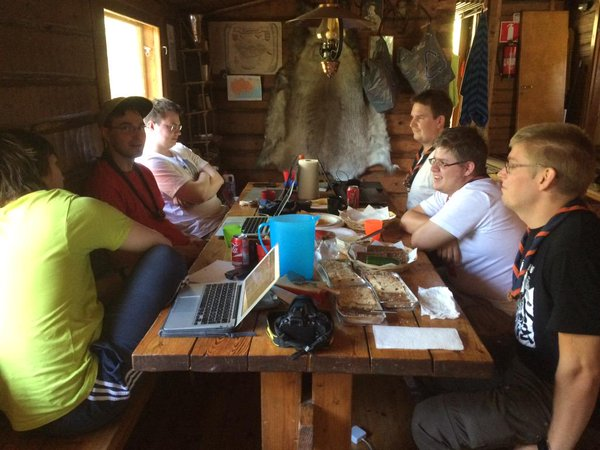
\includegraphics[height=7cm]{kokous.jpg}
	\end{center}
	\caption*{\textbf{Toiminnansuunnittelua lippukunnan kämpällä.}}
\end{figure}


Ryhmät koontuivat omiin tapaamisiinsa viikoittain ja johtajat pitivät omia kokouksiaan tarpeen mukaan, esimerkiksi retkien suunnittelua varten. Kokouksista ja niiden määrästä lista alla:\\
\begin{center}
	\begin{tabular}{ l l }
		Vuosikokous & 1 kpl\\
		Vaalikokous & 1 kpl\\
		Hallituksen kokous & 9 kpl\\
		Poikasamoajat & 20 kpl\\
		Poikatarpojat & 20 kpl\\
		Poikasudenpennut & 50 kpl\\
		Tyttötarpojat & 25 kpl\\
		Tyttöseikkailijat & 25 kpl\\
		Tyttösudenpennut & 25 kpl\\
			      & \\
		\textbf{Yhteensä} & \textbf{176 kpl}\\
	\end{tabular}
\end{center}
Lisäksi vuoden mittaan on pidettu lukuisia muita pienempiä ja epävirallisia kokouksia, joissa on esimerkiksi suunniteltu toimintaa, retkiä tai kämppien kunnostusta.
\subsection{Leirit ja retket}
\subsubsection{Jouluretki}
Joulukuussa 2015 Helsingin Kotkat järjesti kaksi yötä kestäneen talviretki Tontun. Retkenjohtajina toimivat yhdessä Jukka Holopainen ja hänen kaksoisveljensä Pekka Holopainen. Retken teemana toimi tonttuilu ja viikonlopun aikana suunnistettiin, harjoiteltiin partio- ja kädentaitoja sekä kehitettiin lasten esiintymistaitoja. Lisäksi retkellä annettiin partiolupauksia jokaiselle ikäkaudelle. Retki oli johtajiensa PJ-lopputyö ja sille osallistui 11 johtajaa ja 26 retkeläistä.
\subsubsection{Kevätretki}
Huhtikuussa 2016 järjestettiin lippukunnan perinteinen keväretki, jonka johtajana toimi Adel Gatoui. Retkelle otettiin mukaan kaikki seikkailijoista ylöspäin. Tämä johtui siitä, että retkellä ei ollut lainkaan sisämajoitusta ja siellä järjestetty pienoisvaellus oli suhteellisen pitkä. Mukana oli 9 johtajaa ja 16 retkeläistä.
\subsubsection{SuSe-leiri}
Tähän juduja kun leiri on pidetty.
\subsubsection{Roihu 2016}
Tähän setti Roihun jälkeen.
\subsubsection{Ryhmien retket}
Lippukunnan ryhmät ja osastot retkeilivät seuraavasti:
\begin{center}
	\begin{tabular}{l l l}
		16.-18.10. & Poikasamoajat Willassa & 4 osallistujaa\\
		30.10.-1.11. & Tyttöseikkailijoiden retki & 10 osallistujaa\\
		11.-13.3. & Tyttöosaston retki & 21 osallistujaa\\
	\end{tabular}
\end{center}
\subsection{Muu toiminta}
\subsubsection{Kisat}
Helsingin Kotkaista oli edustajat lähes jokaisissa pääkaupunkiseudulla järjestetyissä partiotaitokilpailussa. Mainetta ja kunniaa ei niistä kummemmin niitetty, mutta niissä edustaneiden lippukuntalaisten partiotaidot kasvoivat ja kehittyivät henkisen kasvun ja partioaatteen ymmärtämisen ohella.
\subsubsection{Kurssit ja koulutus}
Lippukuntalaiset kävivät tällä toimikaudella poikkeuksellisen paljon johtajakoulutusta. Partionjohtajakurssilla ja ryhmänohjaajakurssilla oli molemmilla kaksi edustajaa.
\subsubsection{Muuta}
Helsingin Kotkat on tehnyt aktiivisesti yhteistyötä Mellunkylän seurakunnan ja Mellunmäki-Seuran kanssa.\\ 
\\Itsenäisyyspäivänä Helsingin Kotkat nostivat lipun Lions Clubin tapahtumassa ja osallistuivat Mellunmäen ostarilla järjestettävään itsenäisyyspäivän tilaisuuteen. Lippukunta nosti itsenäisyyspäivänä lipun myös Mikaelinkirkolla ja osallistui itsenäisyyspäivän messuun
\newpage
\section{Toimitilat}
\subsection{Kolo}
Lippukunnan pääasiallisena toimitilana, eli Kolona toimii Mellunmäki-Seuralta vuokrattu noin 50 neliömetrin kokoinen huone. Tilassa olevaa keittiötä alivuokrataan Hilkka Harjulle, joka käyttää tilaa päivisin.
\subsection{Varasto}
Lipukunnan retki- ja leirikalustoa säilytetään Sallatunturintie 1:ssä, jossa lippukunnalla on noin 30 neliömetrin kokoinen varastotila. 
\subsection{Willa}
Lippukunnan käytössä on Nuuksiossa yksityisellä luonnonsuojelualueella sijaitseva Willa-niminen kämppä. Kämpälle tehdään ryhmien toimesta retkiä muutaman kerran vuodessa. Kämpästä ei makseta vuokraa.
\subsection{Kyöpeli}
Lippukunnan pääasiallisena kämppänä toimii osoitteessa Ruuhijärventie 17 sijaitseva Kyöpeli. Kämppään kuuluu laajahko tontti. Kämppää käytetään lippukunnan omiin retkiin ulkopuolelle vuokrauksen lisäksi. Myös lippukunta maksaa omista retkistään vuokraa, jotta kämpän ylläpitoon saadaan riittävästi varoja.\\
\\Kämpän suhteen tehdään läheistä yhteistyötä Paakaupunkiseudun partiolaisten kanssa. Tämä näkyy siten, että lippukunnalla on 1/4-osa käyttöoikeus kaikkiin piirin tarjoamiin palveluihin. Näihin kuuluu sauna, vesikaivo ja jätehuolto.\\
\\Kyöpelillä vietetään joka vuosi talkoot, yleensä Helatorstaina. Tällä toimikaudella talkoissa tehtiin valtavat määrät puutöitä sekä uudet penkit nuotiopaikalle, lisäksi sisätiloissa tehtiin parannustöitä keittiöön.
\newpage
\section{Jäsenet}
\newpage
\section{Hallitus ja toimihenkilöt}
\begin{center}
	\begin{tabular}{ l l }
		\textbf{Hallitus} & \\
		Onni Lampi & lippukunnanjohtaja\\
		Hanna Tompuri & lippukunnanjohtajan apulainen\\
		Pyry Aaltonen & sihteeri, uudet jäsenet\\
		Eero Lilja & taloudenhoitaja, jäsenrekisterinhoitaja\\
		Pekka Holopainen & varasto- ja kolovastaava\\
		Heidi Ekblom & koulutusvastaava, viestintämestari\\
		Pauli Saarikoski & ohjelmavastaava\\
		Aapo Launiainen & kämppävastaava\\
					      & \\
		\textbf{Muut toimihenkilöt} & \\
		Kimmo Huurinainen & kirjanpitäjä\\
		Ari Söderqvist & toiminnantarkastaja\\
		Minna Söderqvist & varatoiminnantarkastaja\\
						& \\
		\textbf{Ryhmät ja niiden johtajat} & \\
		Uudet poikasudenpennut & Ikra Sheikh, Jenni Halkola, Tanja Kaappola\\
		Vanhat Poikasudenpennut & Hanna Tompuri, Heidi Ekblom\\
		Poikatarpojat & Pauli Saarikosi, Pyry Aaltonen\\
		Tyttöseikkailijat & Ikra Sheikh, Jenni Halkola, Tanja Kaappola\\
		Poikasamoajat & Adel Gatoui\\
		Tyttösudenpennut & Mari Aho(?)\\
		Tyttötarpojat & Aino Pirskanen, Elli Kasvi\\
	\end{tabular}
\end{center}

\newpage
\section{Talous}
Lippukunta on säilynyt vakavaraisena läpi tilikauden. Lippukunta sai Urlus-säätiöltä 5000\euro{} avustusta Kyöpelin katon uusimiseen, tämä toteutetaan <joskus>. Lippukunta haki ja sai myös 1500\euro{} rahaa leirikalustonsa uusimiseen, tällä hankittiin uusi puolijoukkueteltta. Varoja koitetaan säästää tulevaisuutta varten, esimerkiksi suojaamaan nousevalta toimitilavuokralta.\\
\\Varainhankintaa toteutettiin perinteisin keinoin. Näihin kuuluivat esimerkiksi adventtikalentereiden myyminen sekä osallistuminen Lions Clubin ja Mellunmäki-seuran tapahtumiin.\\
\\Kyöpelin suhteen varoja kerätään aktiivisesti vuokratuloilla. Vuokratulot käytetään pääsääntöisesti kiinteistön kunnostamiseen ja muihin huoltotoimenpiteisiin. Lippukunta sai myös 5000\euro{} apurahan Urlus-säätiöltä kattoremonttia varten ja noin saman suuruisen summan osana Haapakerttujen viime vuotista lahjakirjaa. Viimeisenä mainittu simma on korvamerkitty Kyöpeliä varten, eikä siihen kosketa ilman lippukunnan hallituksen erillistä päätöstä

\newpage
\section{Taustayhteisöt}
\begin{figure}[htb]
	\begin{center}
		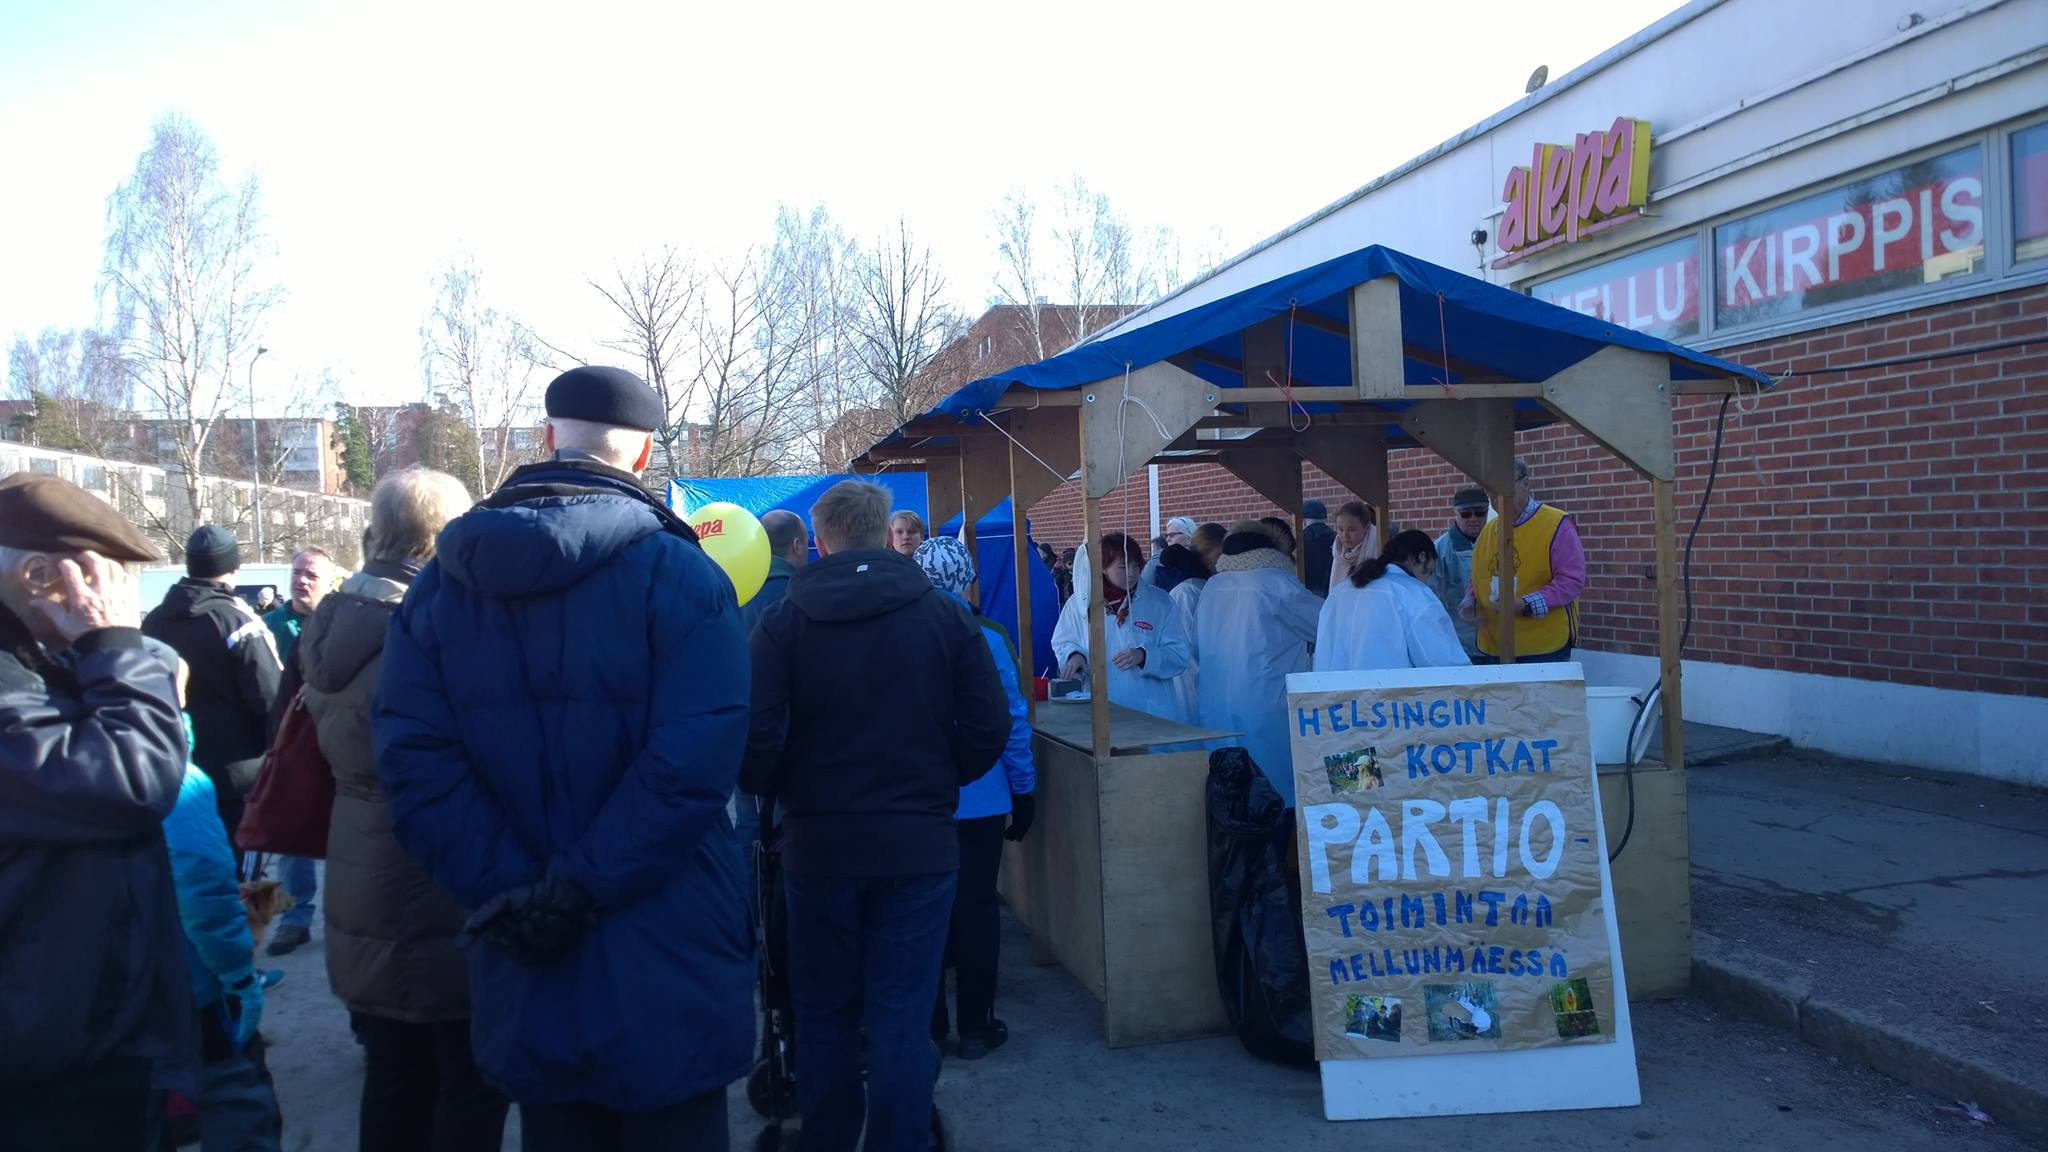
\includegraphics[height=7cm]{lettukestit.jpg}
	\end{center}
	\caption*{\textbf{Vohvelimyyntiä Mellunmäen Lionsien kevätriehassa.}}
\end{figure}

Taustayhteisöinä ovat tuttuun tapaan toimineet Mikaelin seurakunta, Mellunmäen Lions Club ja Partiolippukunta Helsingin Kotkat ry:n Venhempainyhdistys ry. Jokaiseen taustayhteisöön on oltu aktiivisesti yhteydessä ja heidän kanssaan on järjestetty tapahtumia.

\end{document}
